% Copyright © 2015-2016 Martin Ueding <dev@martin-ueding.de>
%
\documentclass[english, fleqn]{beamer}

\usetheme{Dresden}
%\usetheme{Marburg}

\usepackage[bibatend, beamer]{../../header}

\renewcommand\iup{\text i}
\renewcommand\eup{\text e}

\graphicspath{{./}{../Figures/}}

\title{Positron lifetime in metals and insulators}
\subtitle{Experiment K225 -- Universität Bonn}
\author{%
    Martin Ueding
    \and
    Lino Lemmer
}
\date{\daterange{2016-03-24}{2016-03-25}}

\begin{document}

\begin{frame}
    \titlepage
\end{frame}

\begin{frame}
    \frametitle{Literatur}

    \printbibliography
\end{frame}

\section{Theory}

\subsection{Positron sources}

\begin{frame}
\includegraphics{beamer-na22}
\end{frame}

\begin{frame}
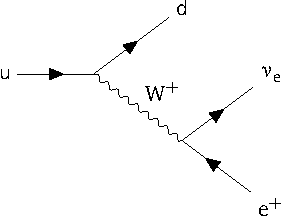
\includegraphics{beamer-beta}
\end{frame}



\subsection{Positron decay}

\begin{frame}
    \frametitle{Decay modes of positrons}

    \begin{columns}[c]
        \begin{column}{.5\textwidth}
            \centering
            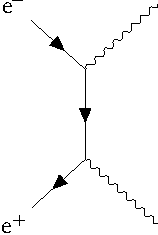
\includegraphics{beamer-two-photon}
        \end{column}
        \begin{column}{.5\textwidth}
            \centering
            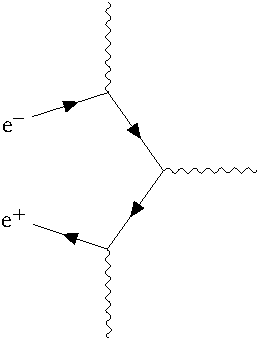
\includegraphics{beamer-three-photon}
        \end{column}
    \end{columns}
\end{frame}



\subsection{Detector and electronics}

\includegraphics{beamer-scheme-176Lu}

\includegraphics{beamer-photomultiplier}

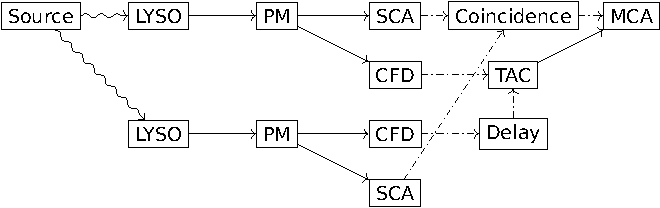
\includegraphics{beamer-fast-slow}

\section{Conduction}

\subsection{Slow circuit setup}

\includegraphics{beamer-lyso-li}

\includegraphics{beamer-lyso-re}

\includegraphics{beamer-na-li}

\includegraphics{beamer-na-re}

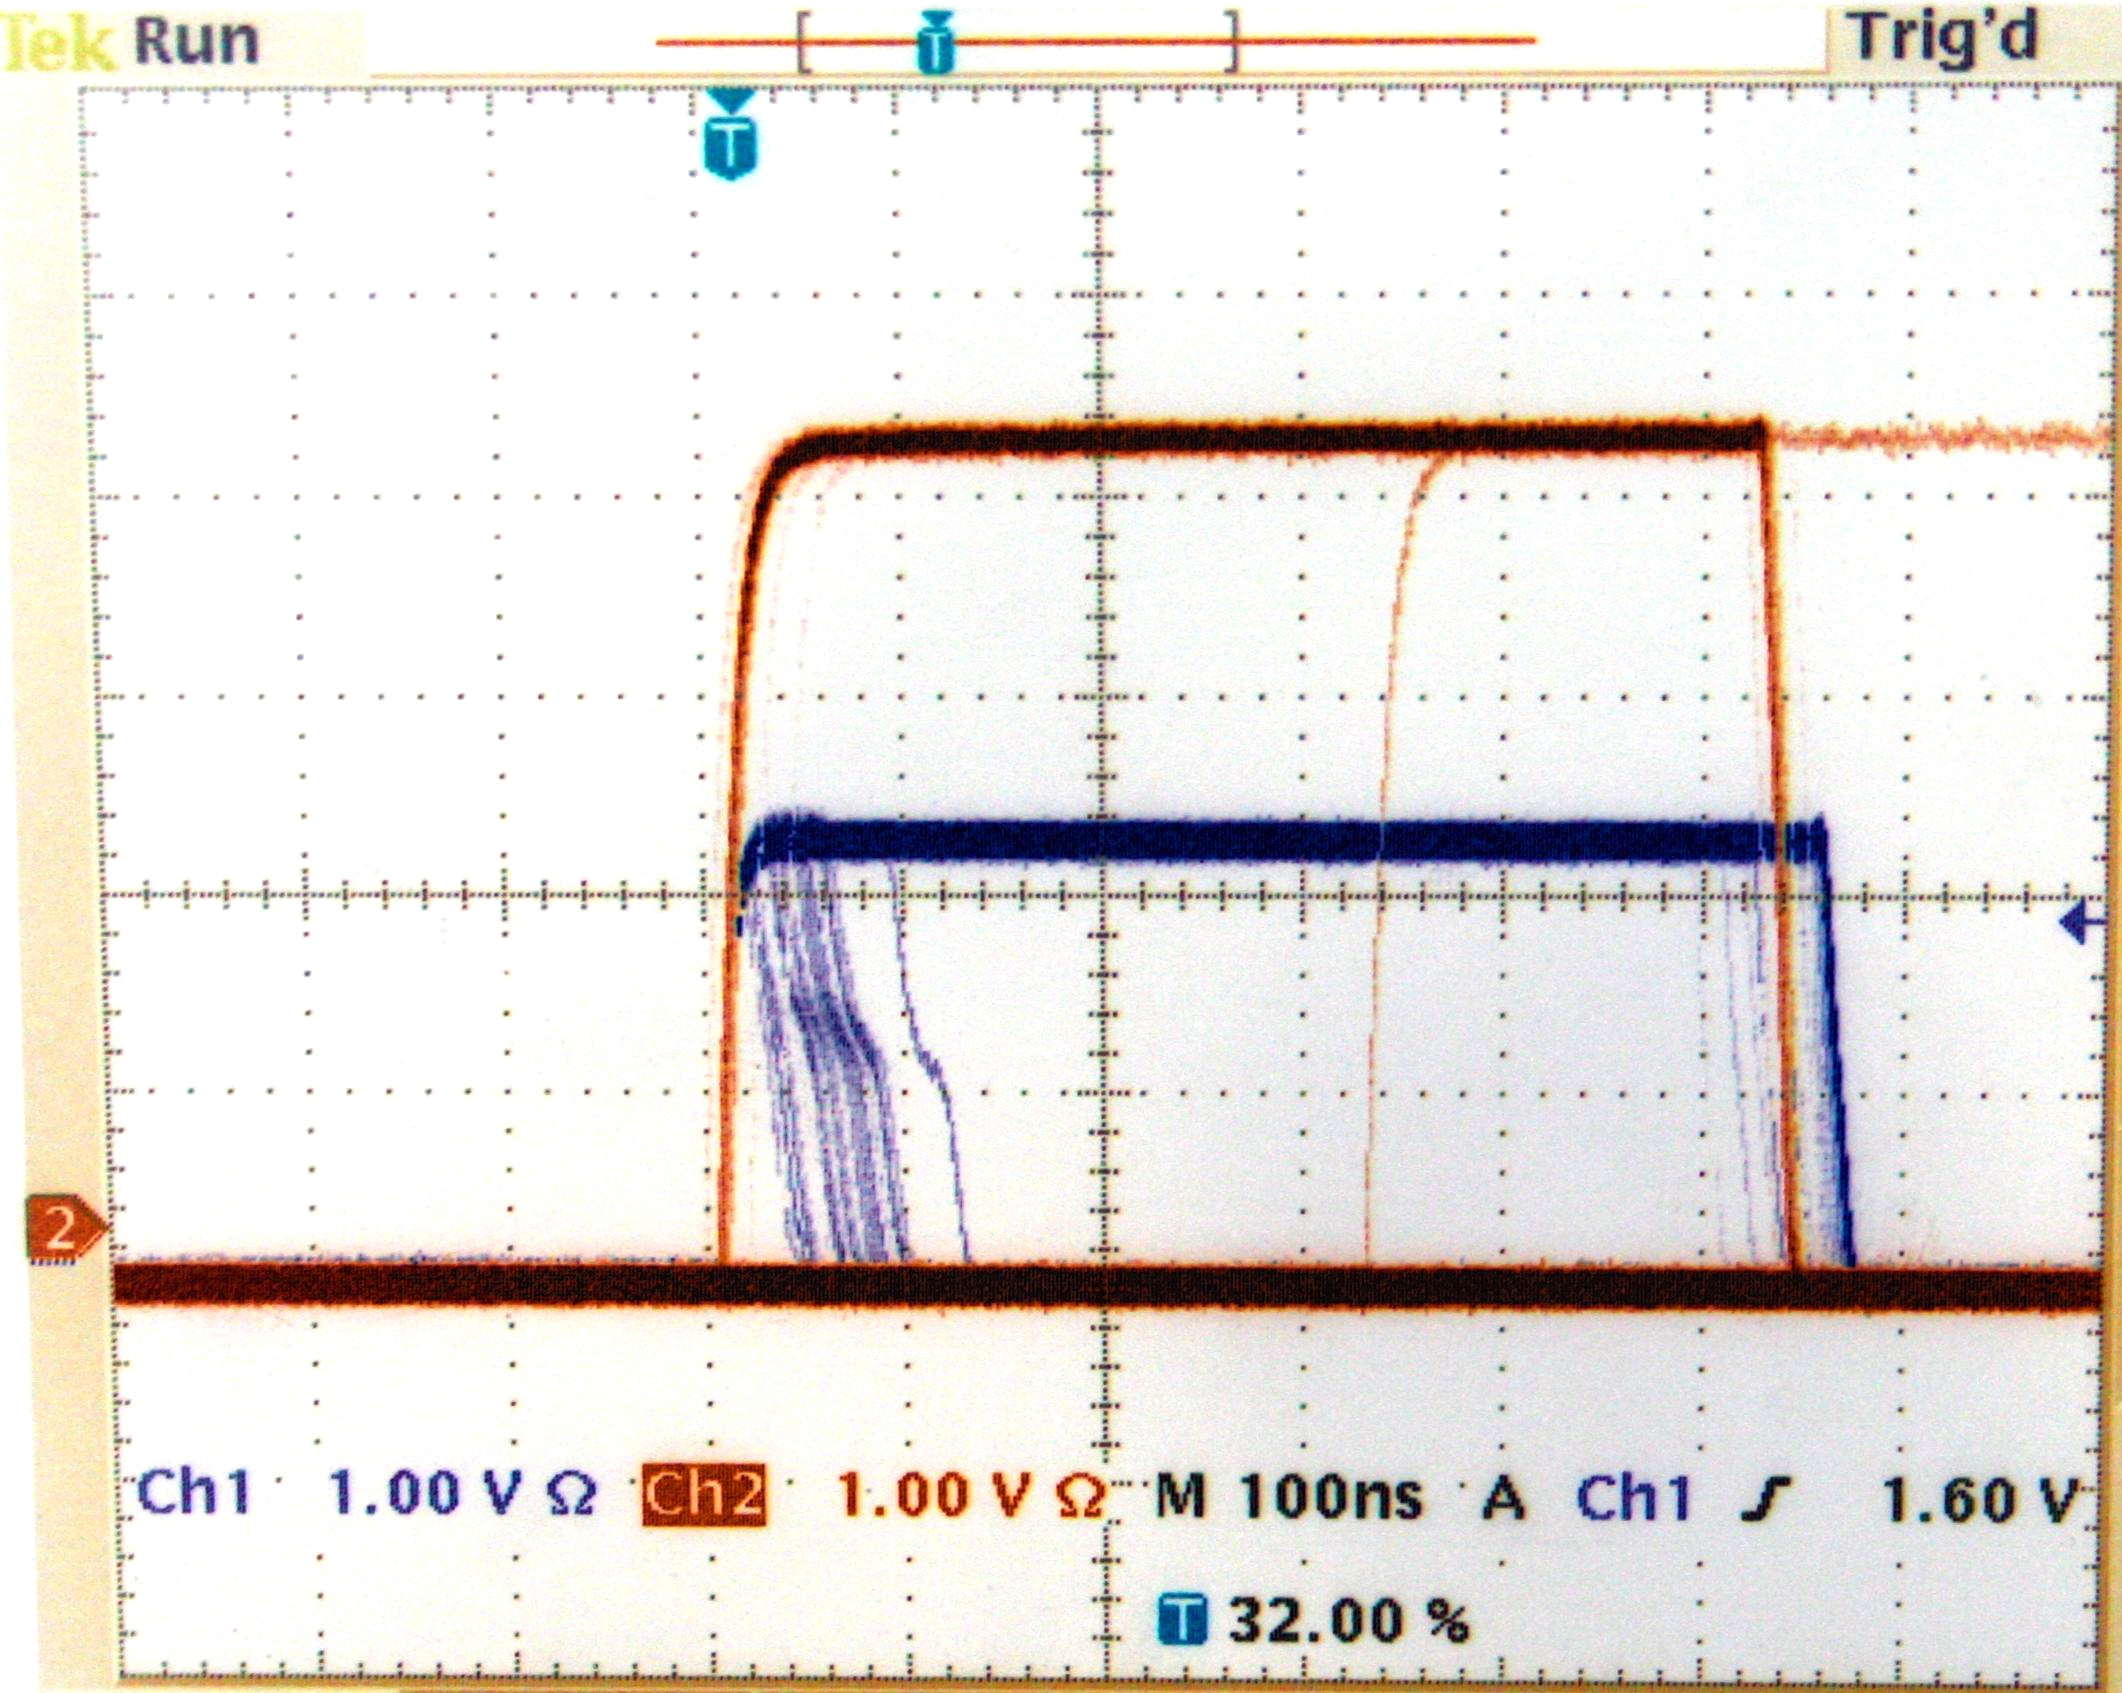
\includegraphics[width=.48\linewidth]{br-1-sca-coincidence-511}

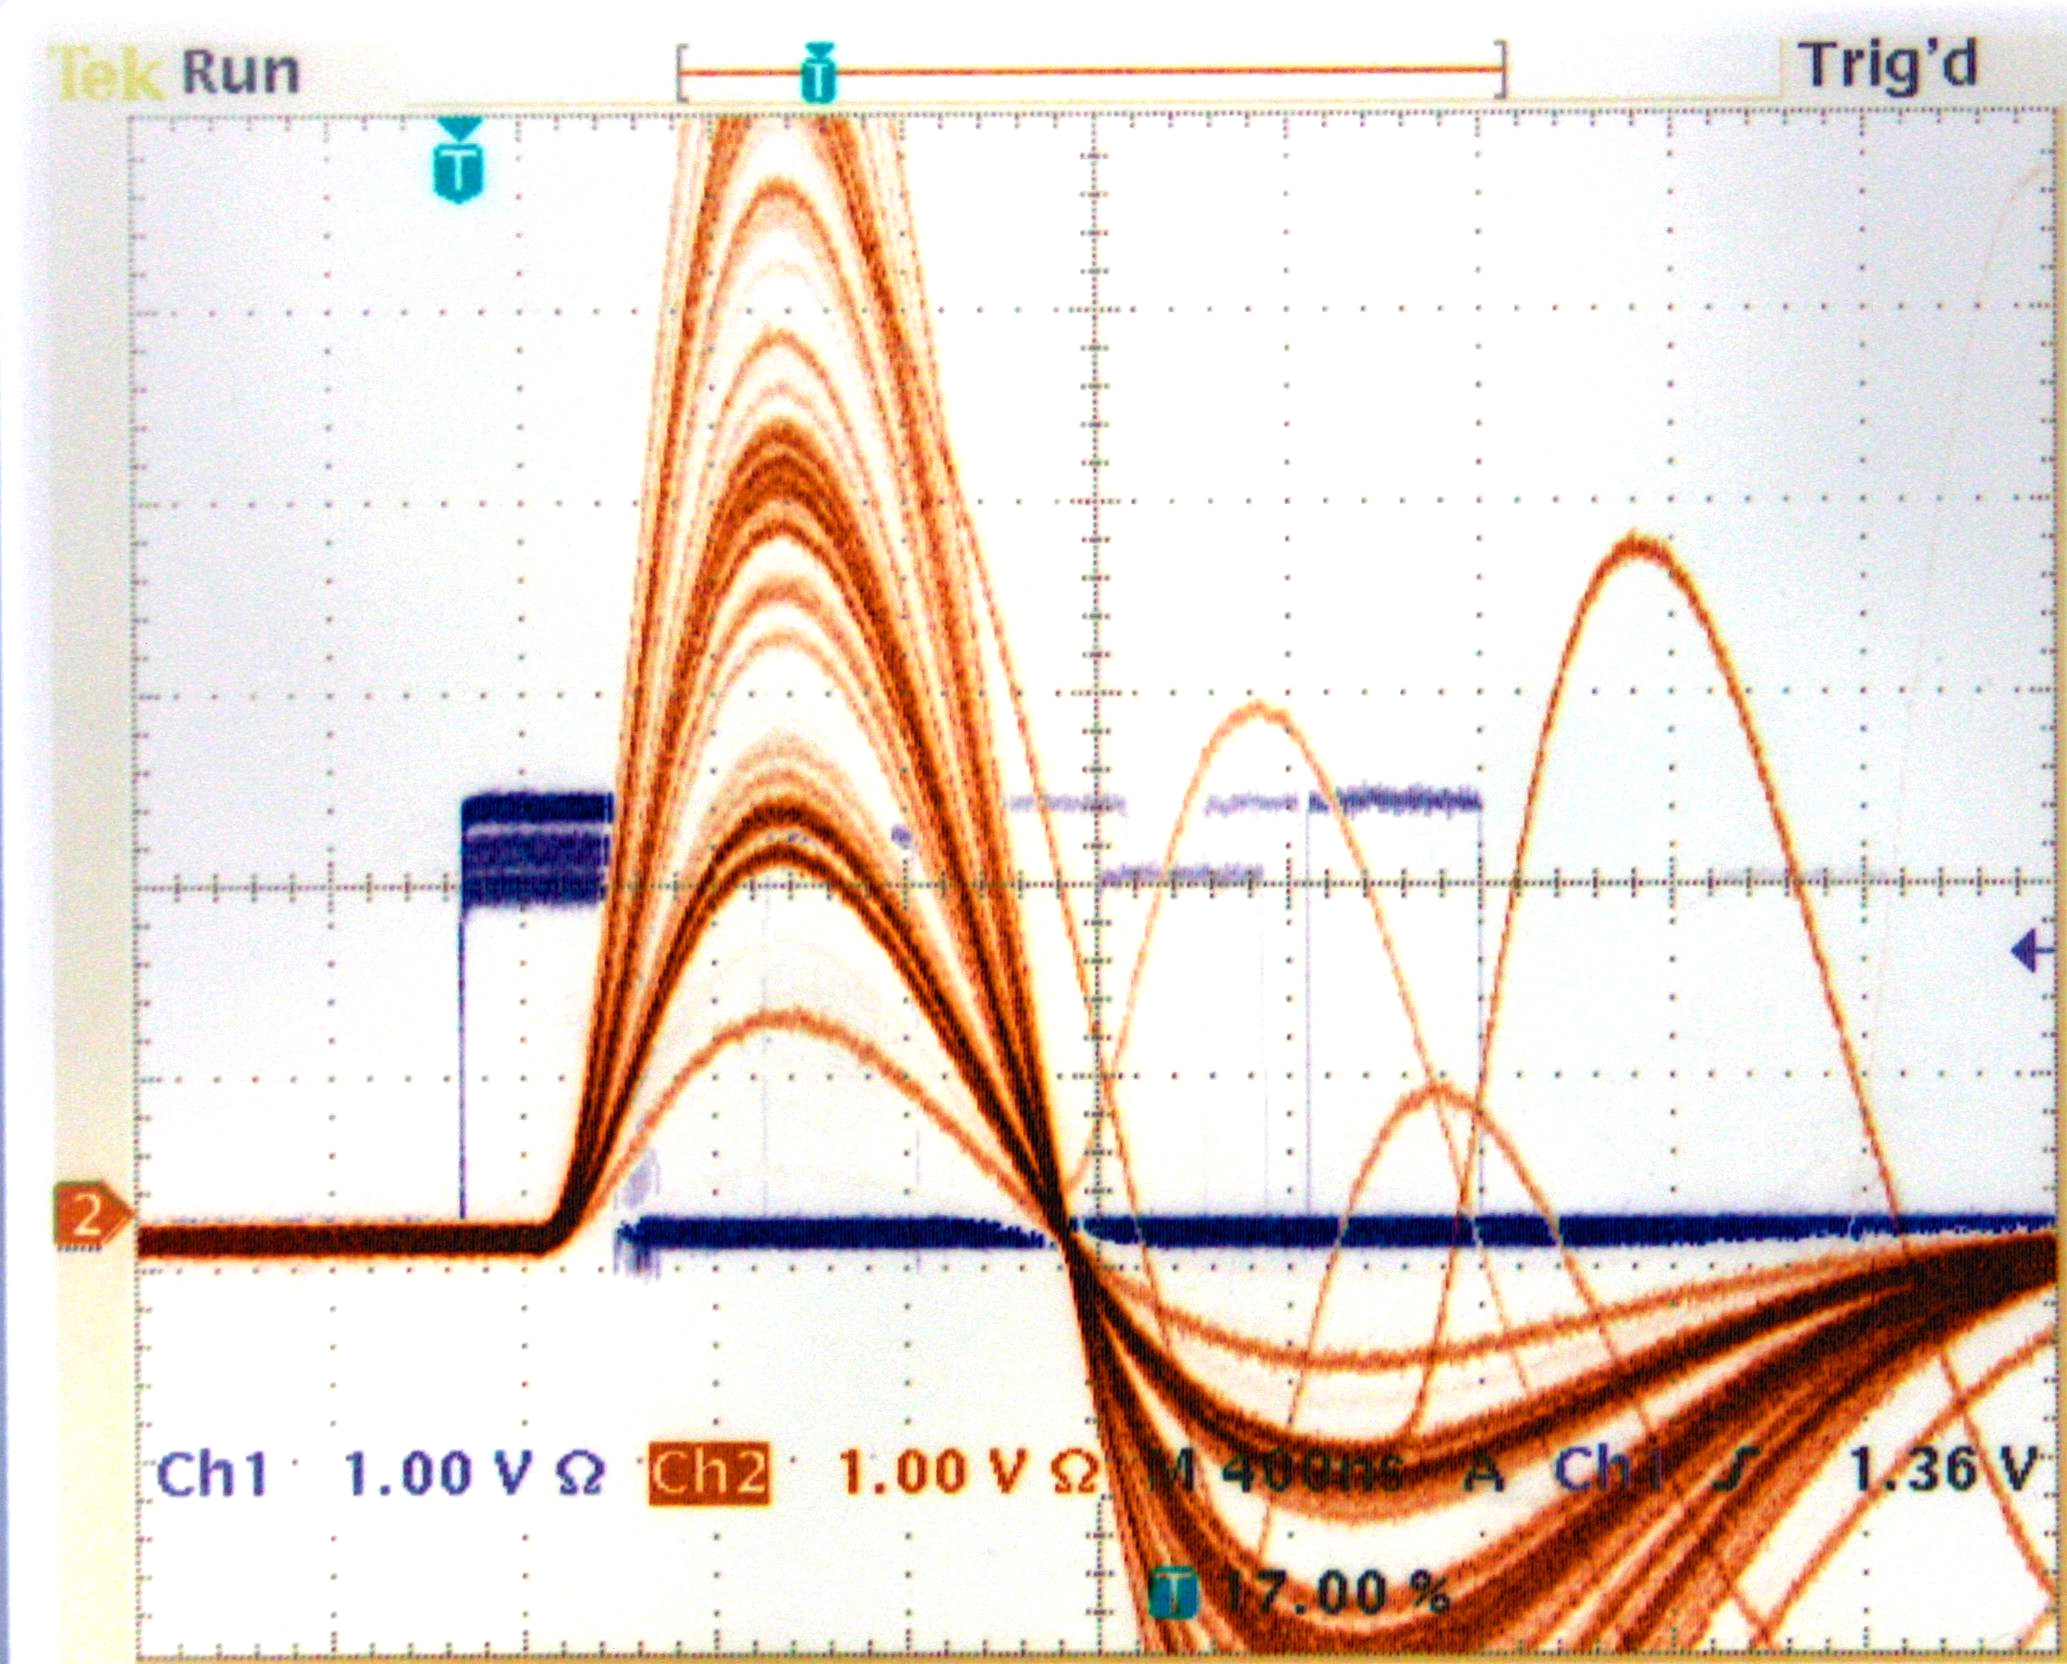
\includegraphics[width=\linewidth]{br-2-sca-and-slow}

\subsection{Fast circuit setup}

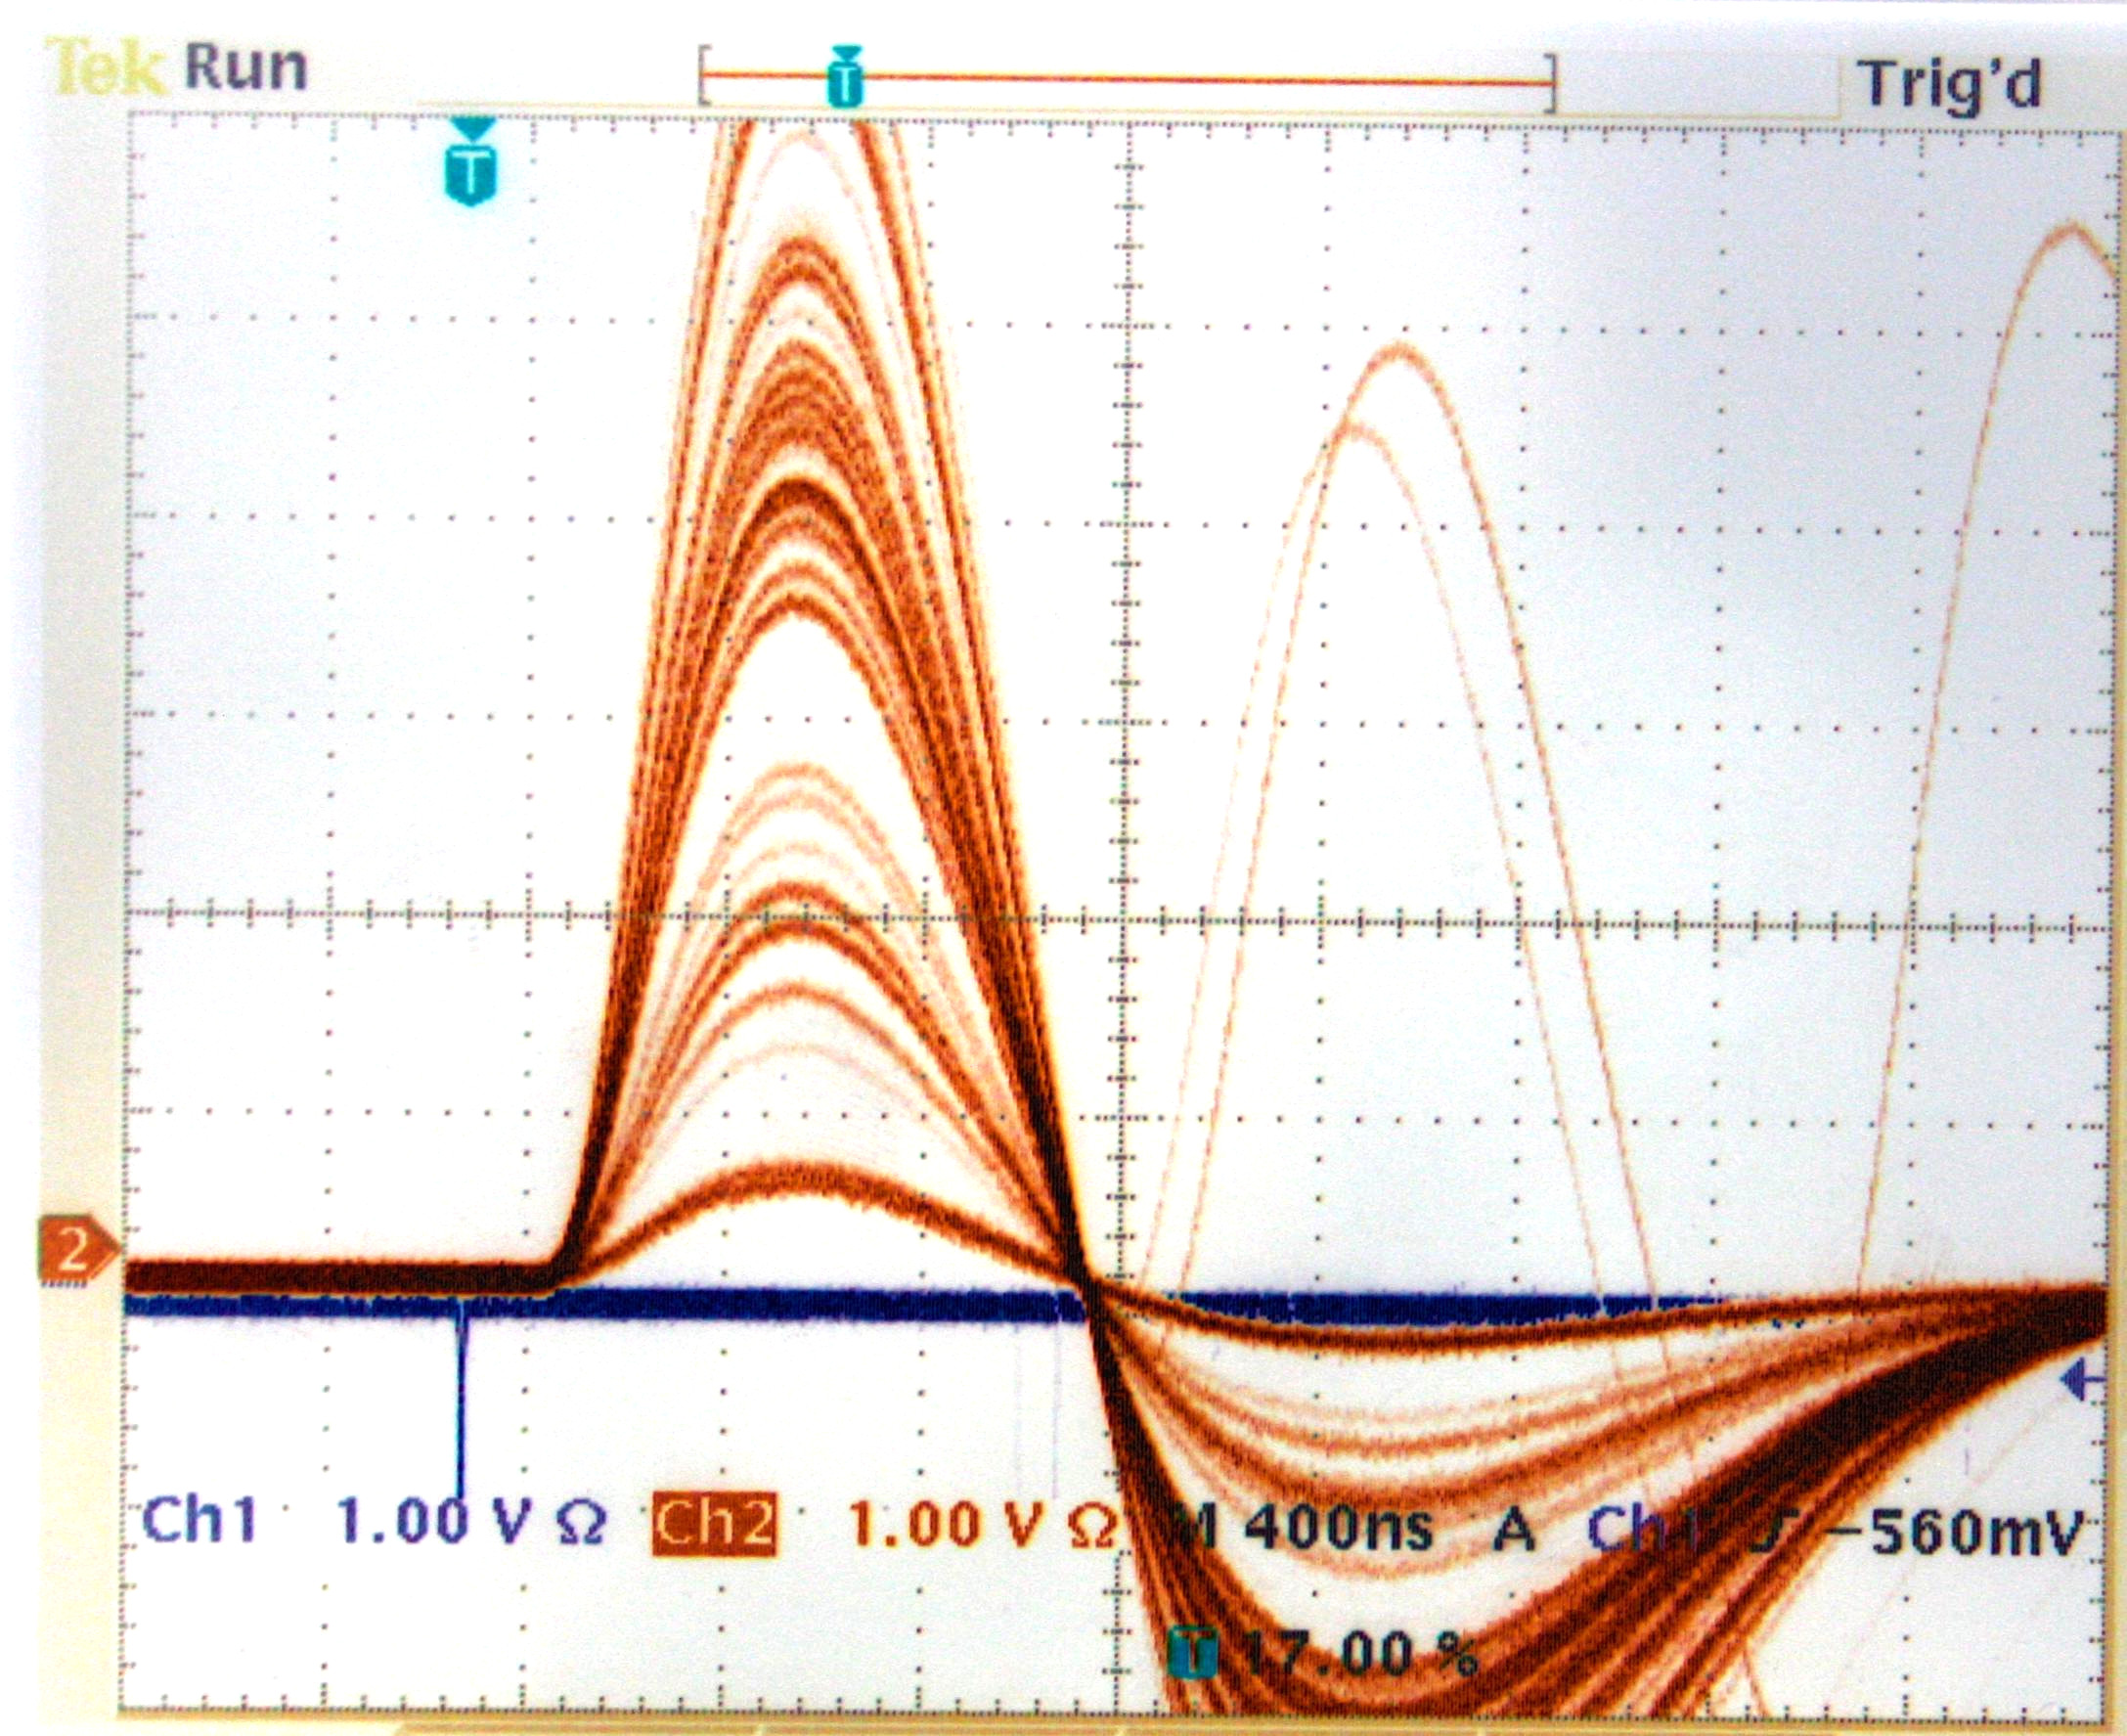
\includegraphics[width=\linewidth]{br-3-cfd-and-slow}

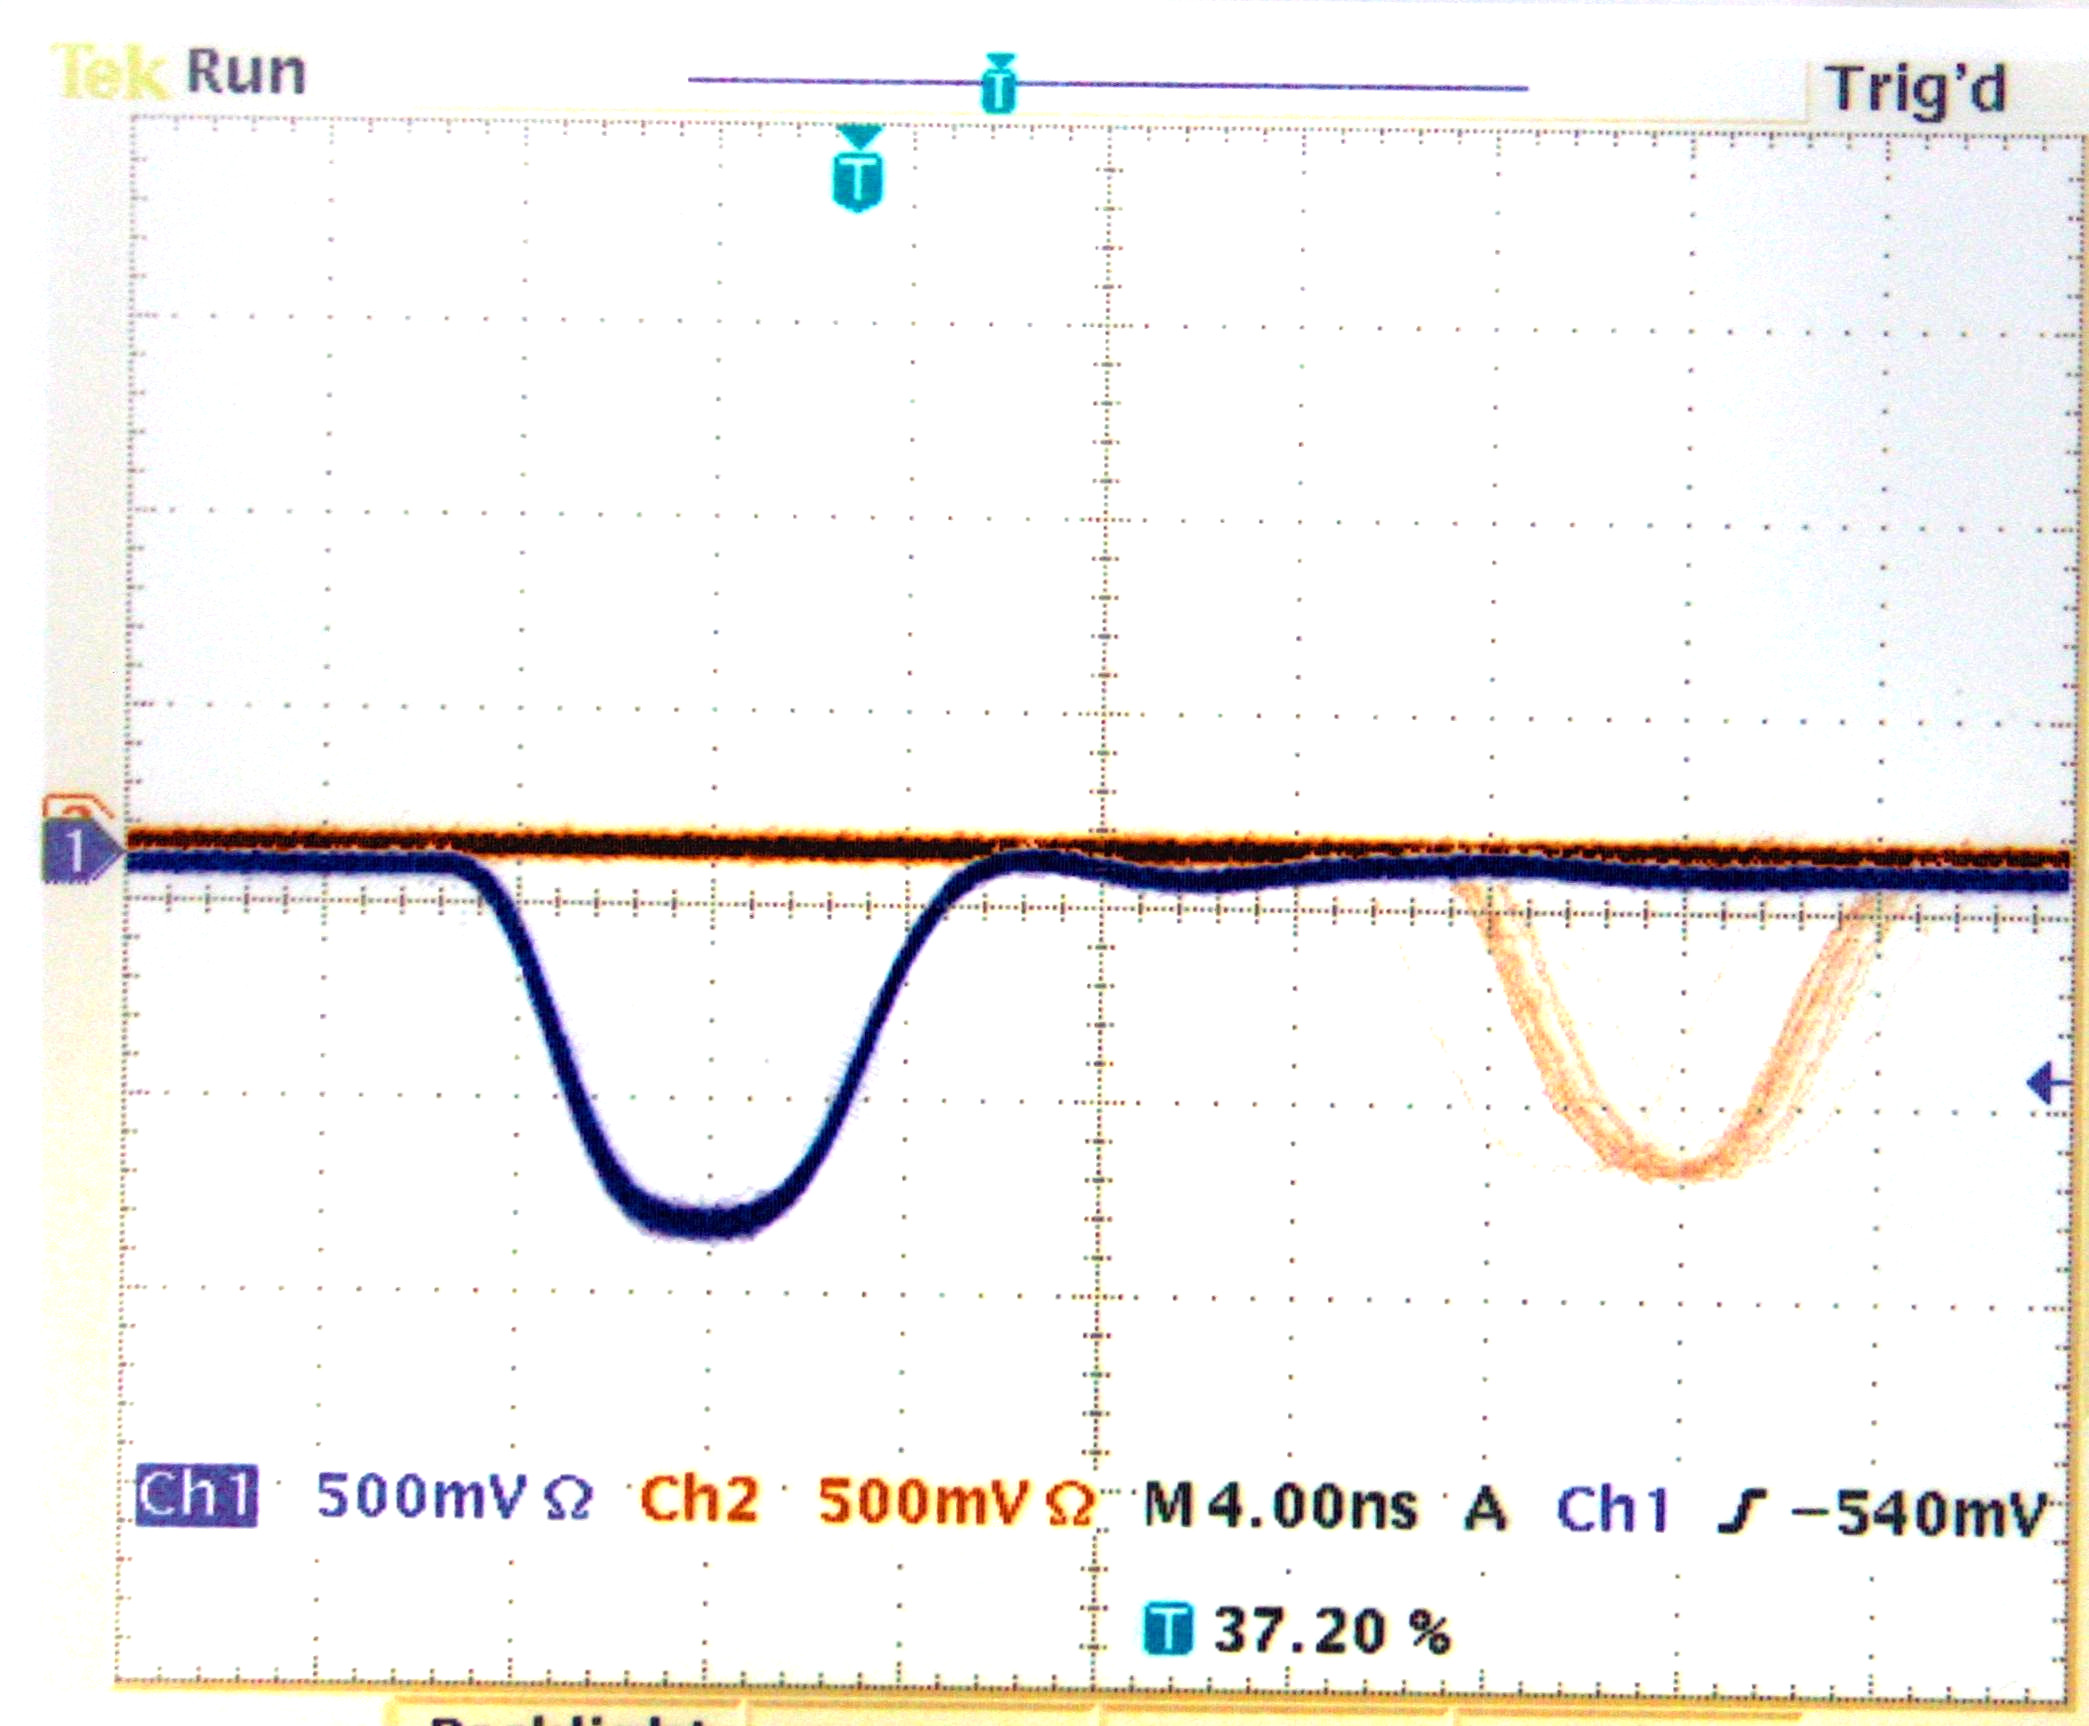
\includegraphics[width=\linewidth]{br-4-cfd-delay}

\subsection{Time calibration}

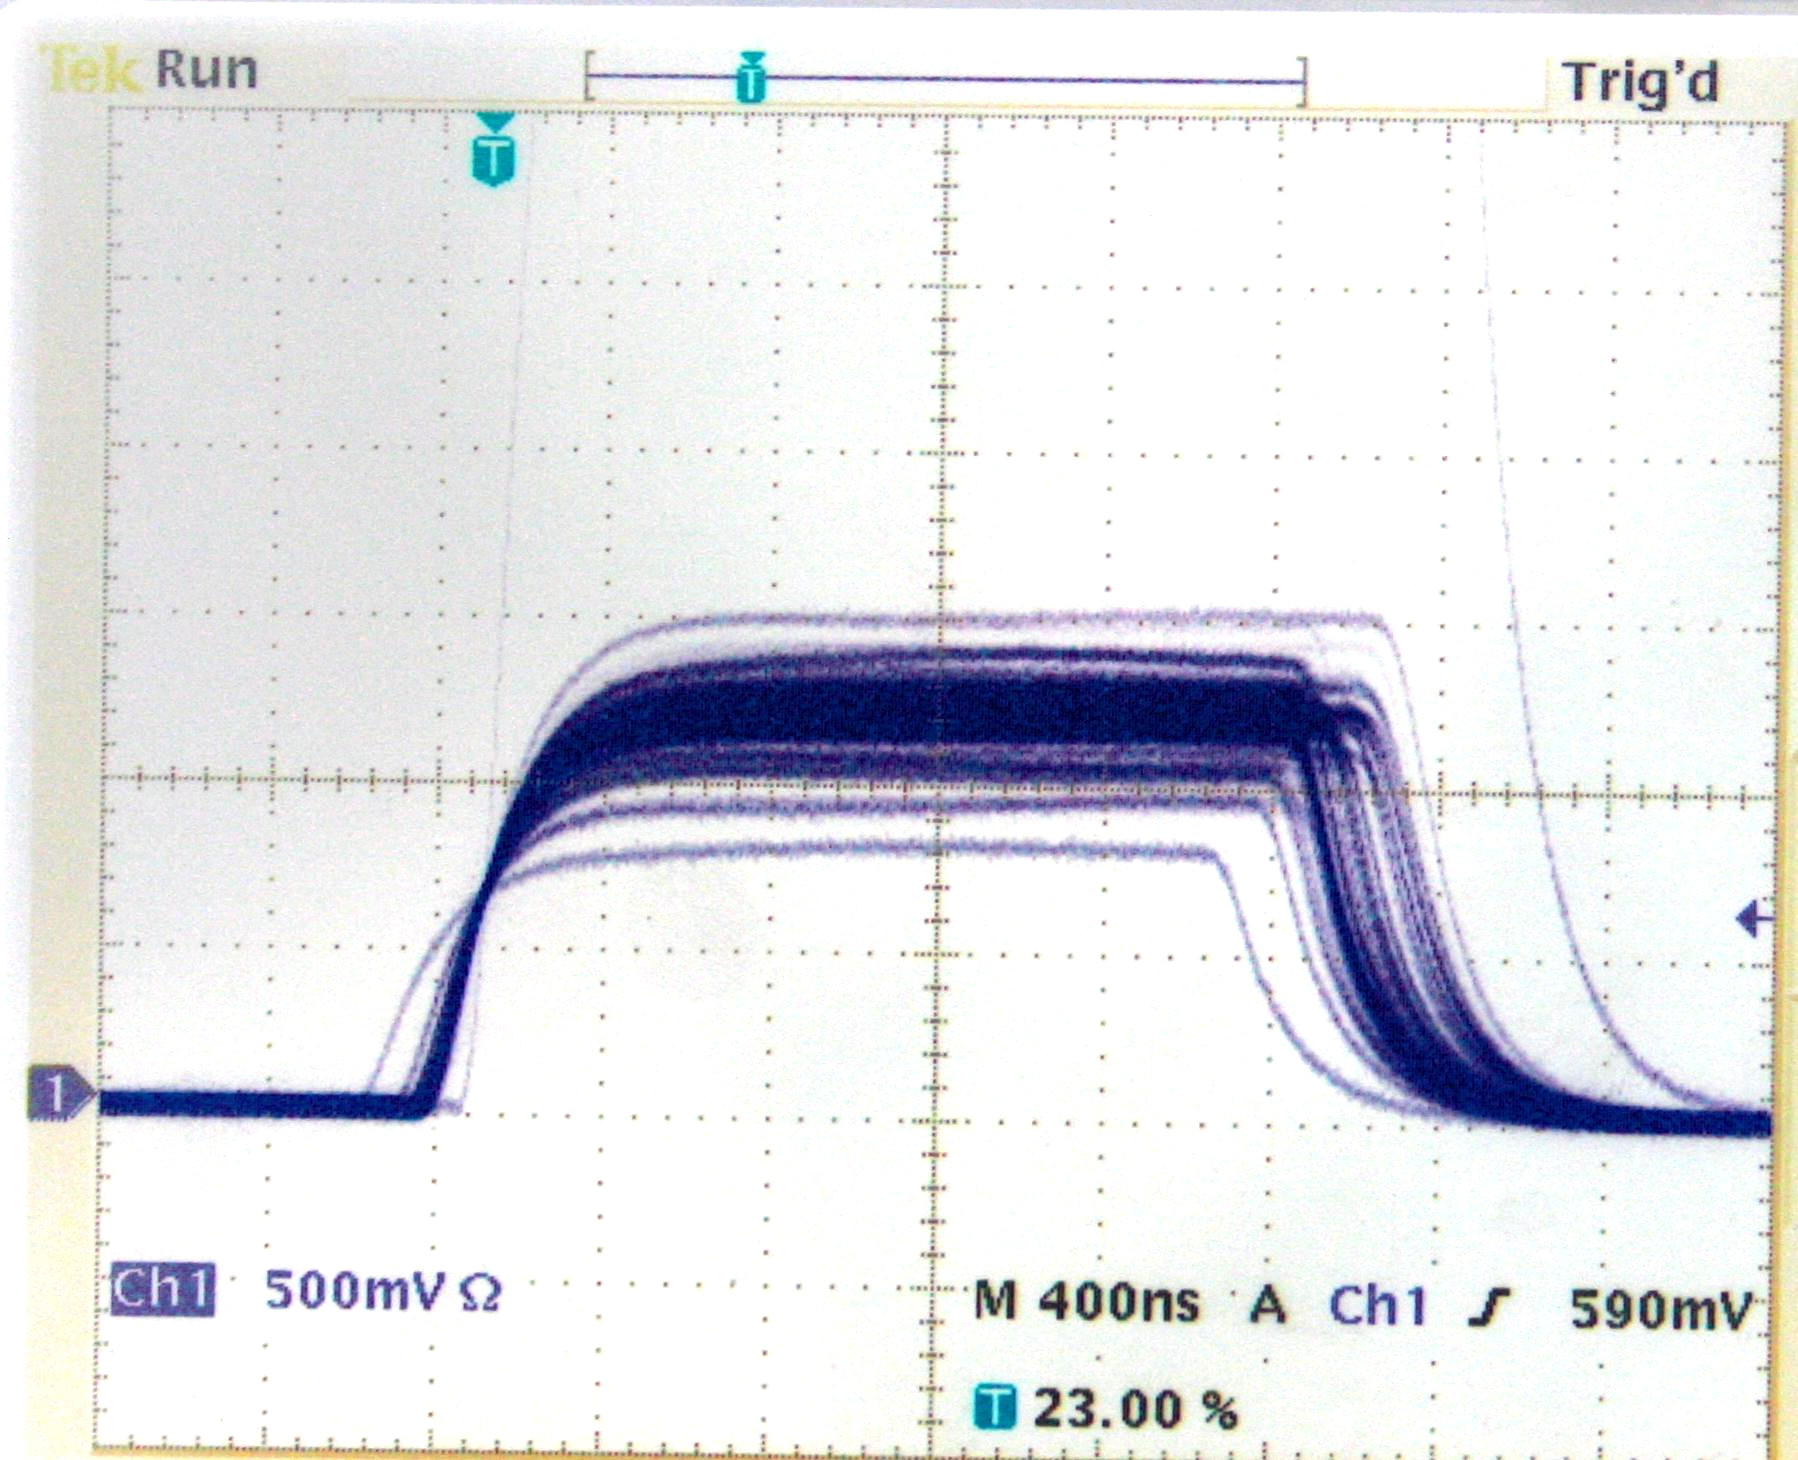
\includegraphics[width=\linewidth]{br-5-tac-511}

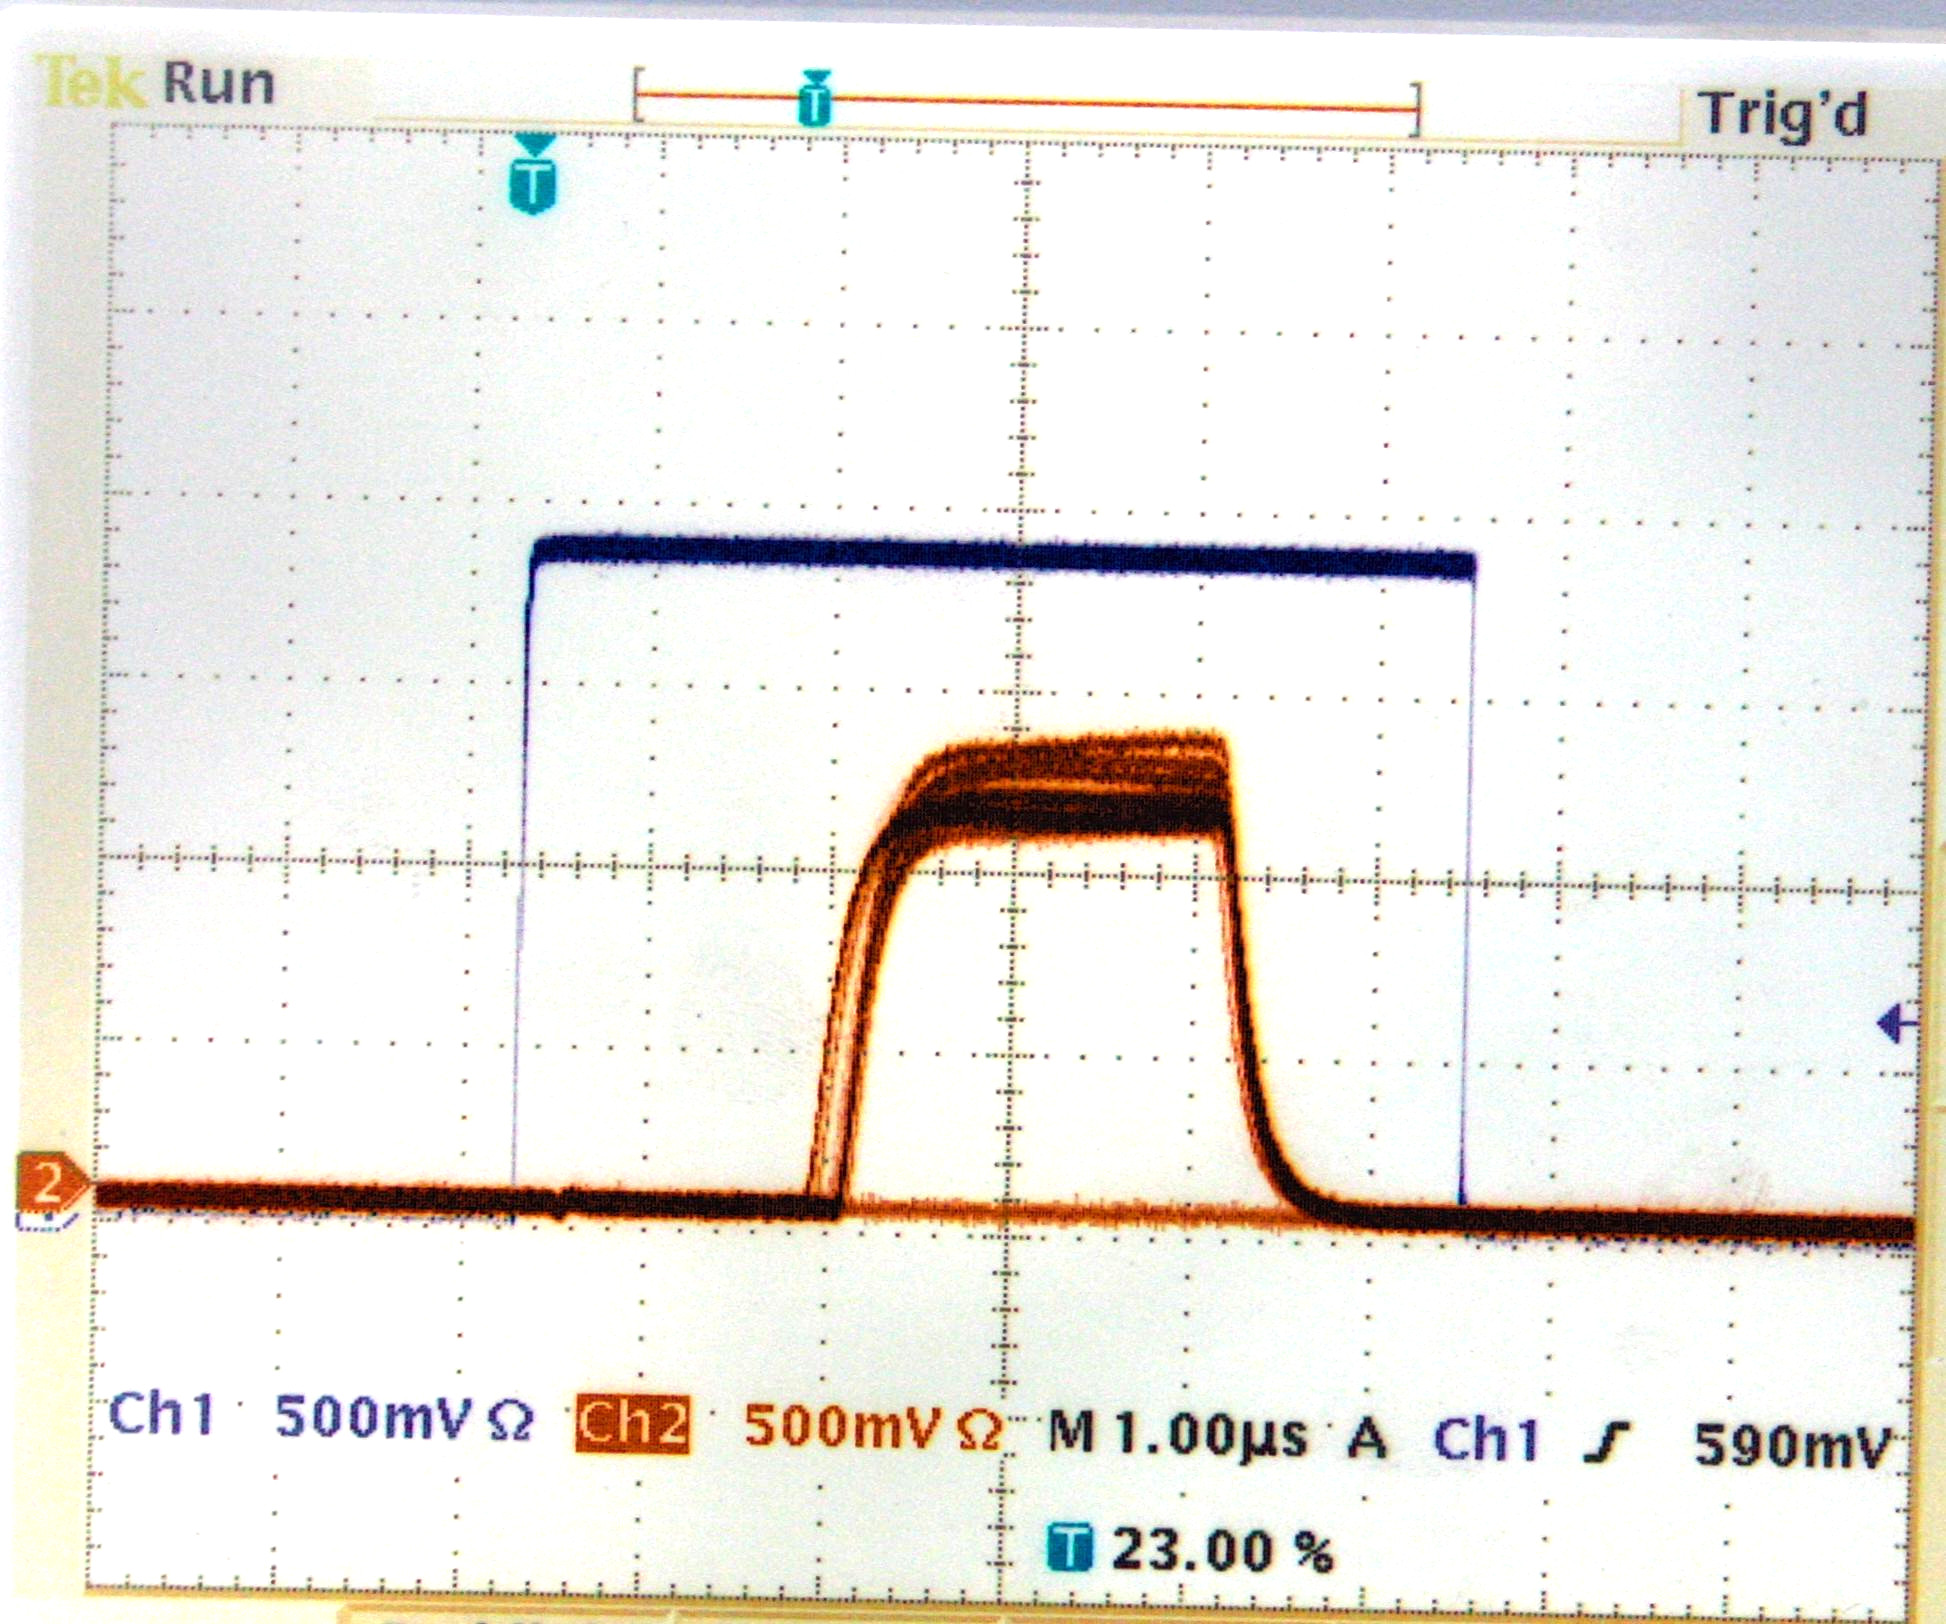
\includegraphics[width=.48\linewidth]{br-6-tac-and-coincidence-511}

\includegraphics{beamer-prompts_short}

\includegraphics{beamer-prompts_long}

\includegraphics{beamer-time_gauge}

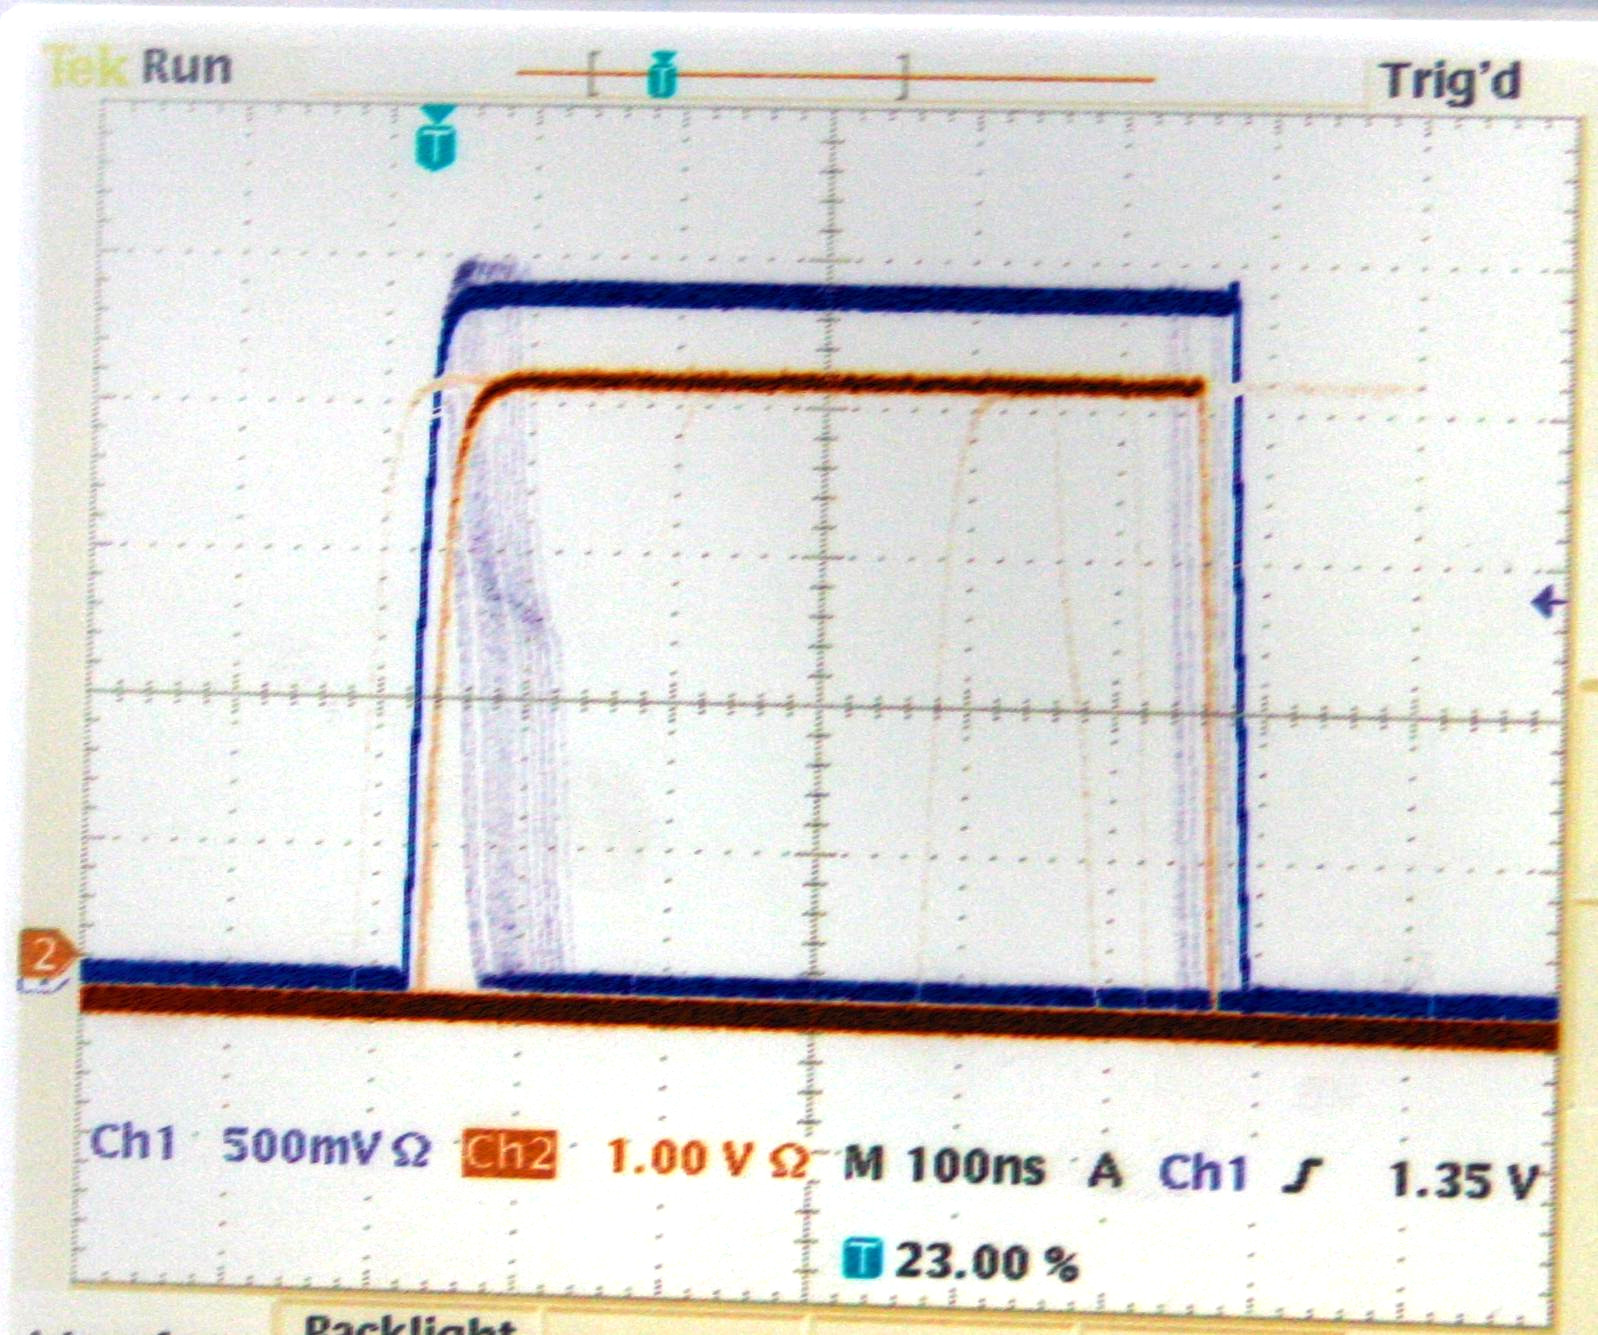
\includegraphics[width=\linewidth]{br-7-sca-coincidence-1275}

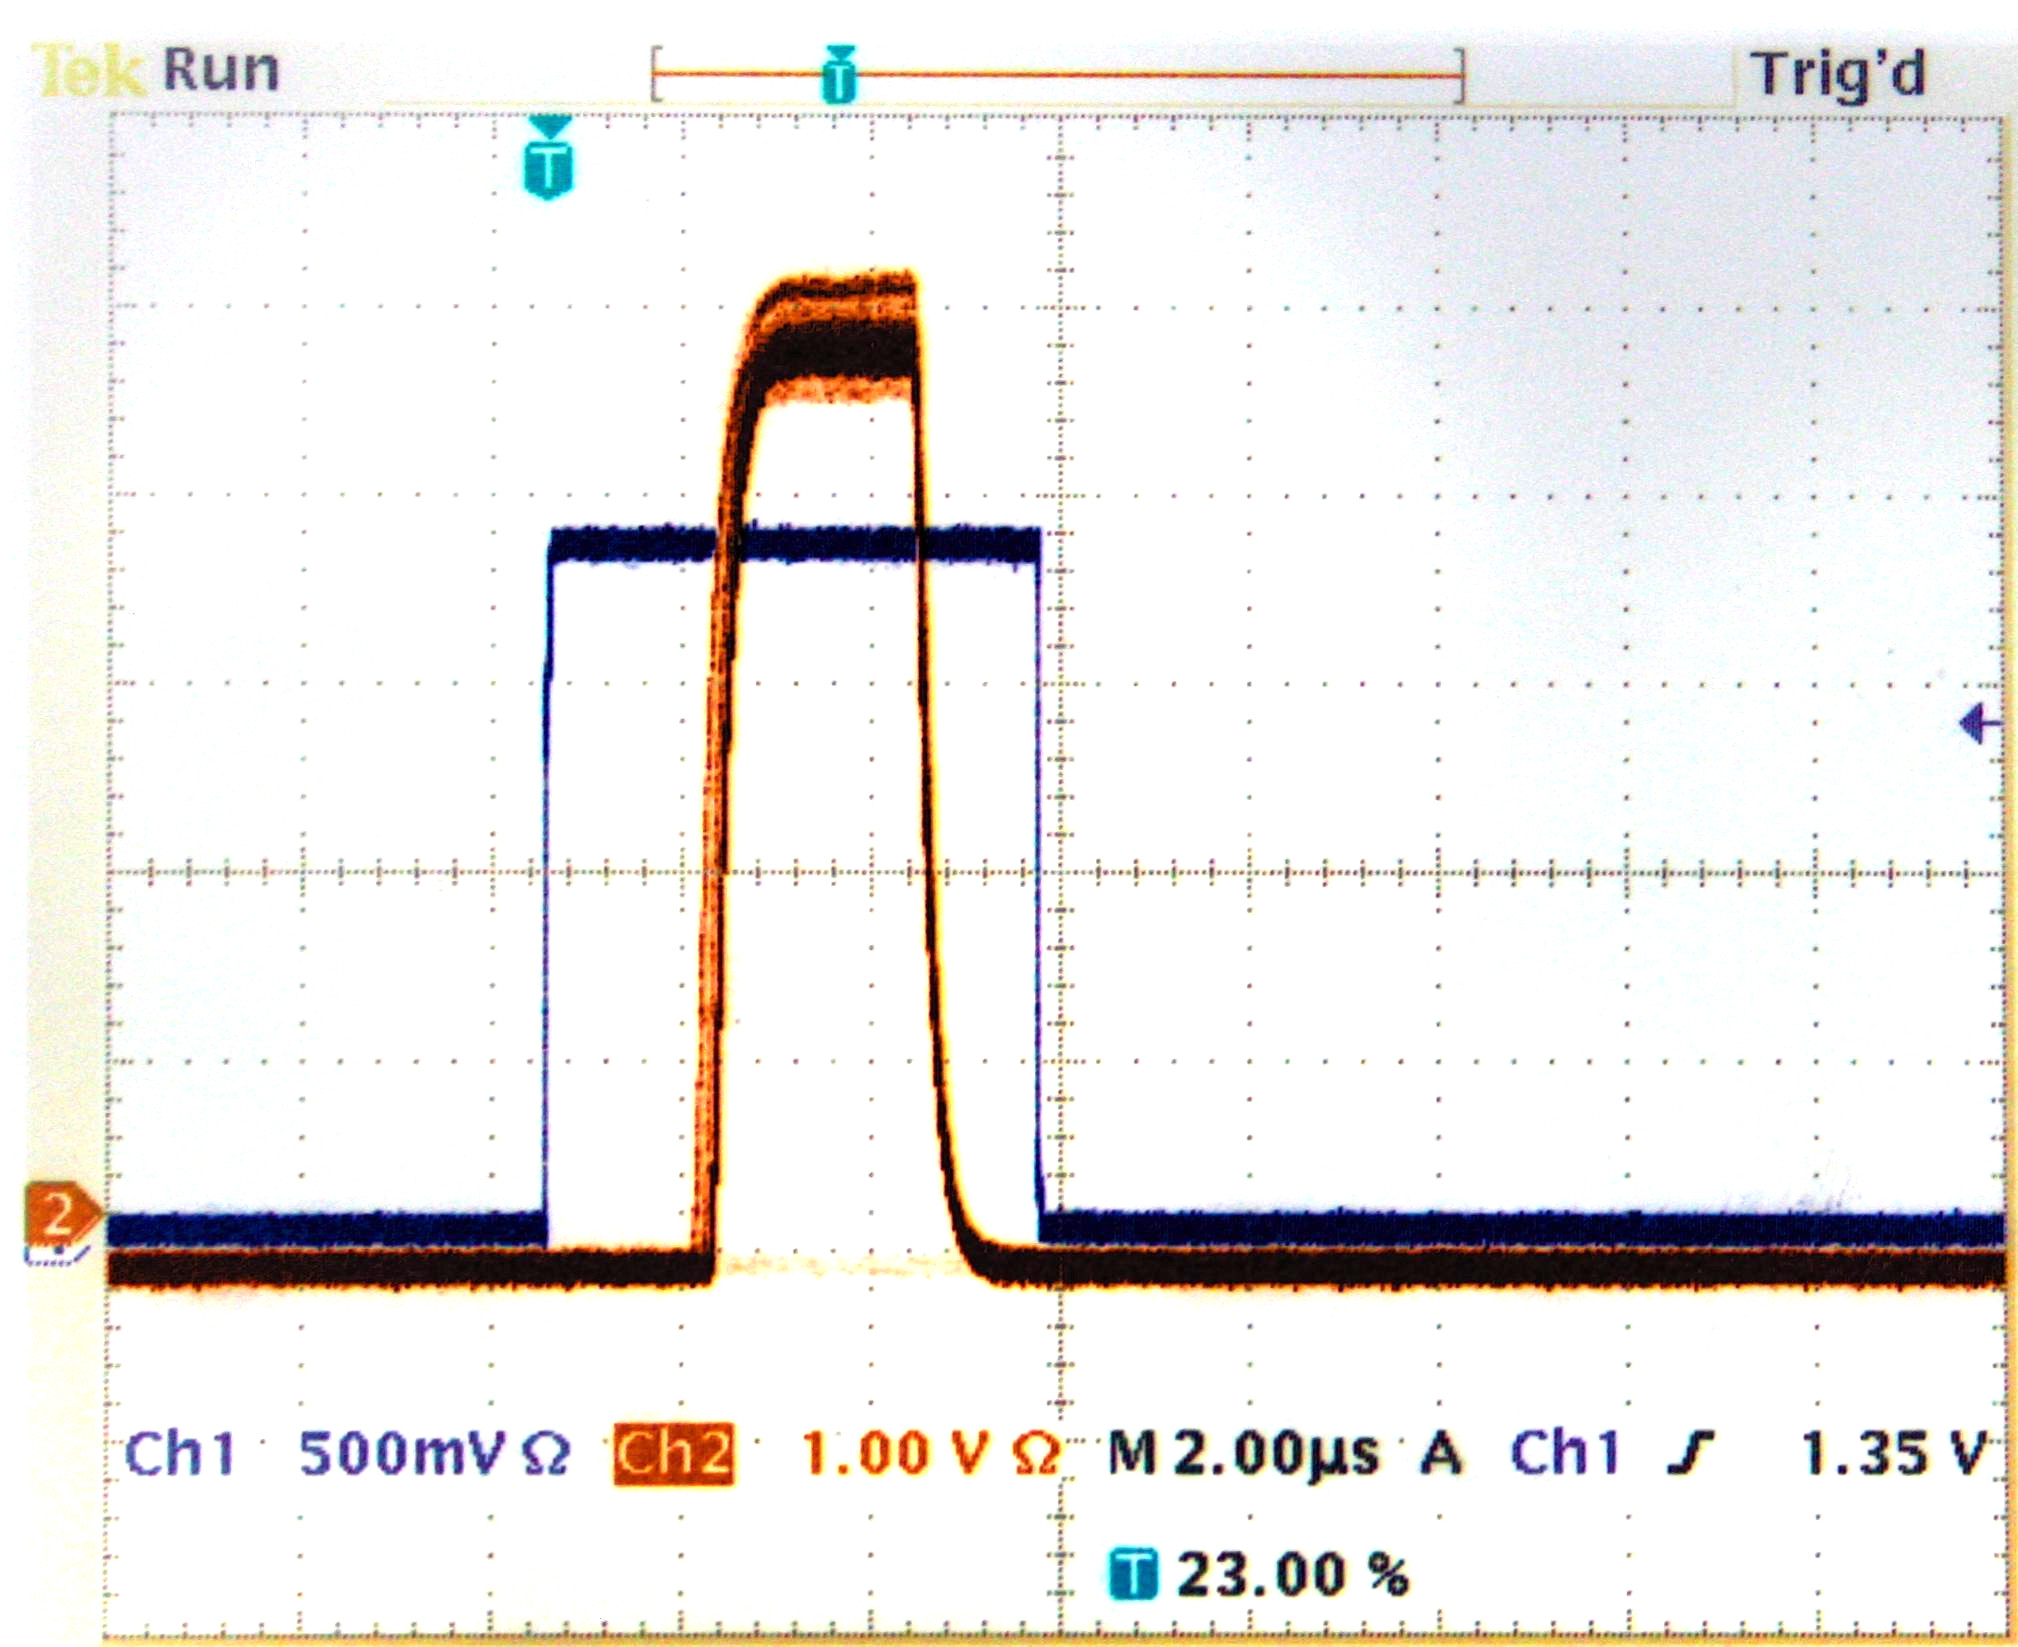
\includegraphics[width=\linewidth]{br-8-tac-and-coincidence-1275}

\subsection{Lifetime measurement}

\includegraphics{beamer-lifetime-295K}

\includegraphics{beamer-acrylic}

\section{Analysis}

\includegraphics{beamer-taus}

\includegraphics{beamer-intensities}

\includegraphics{beamer-s_curve}

\includegraphics{beamer-arrhenius}

\begin{frame}
    \includegraphics{beamer-acrylic-zoom}
\end{frame}

        %\includegraphics{lifetime-<< temp >>K}

% TODO Frame with a picture of the bootstraps on Frederike's boots.

\end{document}

% vim: spell spelllang=en_us
